\subsubsection{Rancangan Detail Subsistem Kontrol}
\label{subsubsection:detail-subsistem-kontrol}
  
Subsistem Kontrol bertanggung jawab mengelola transaksi dan konsistensi antar-\textit{Node}. Pengelolaan tersebut dilakukan dengan mengaplikasikan algoritma konsensus untuk menjaga konsistensi data antar-\textit{Node}. Subsistem ini juga bertanggung jawab untuk melakukan \textit{recovery} data dari \textit{transaction log} jika terjadi kegagalan pada \textit{Node}.

% TODO: Implementasi paxos better masuk bab 2?
Untuk menjaga konsistensi dari data, subsistem kontrol mengimplementasikan algoritma konsensus untuk tiap transaksinya. Algoritma yang dipakai adalah algoritma \textit{Paxos} karena algoritma ini bersifat transaksional dan \textit{message passing} dan bukan \textit{log replication} sehingga lebih ideal untuk sistem yang menggunakan \textit{erasure coding}.

Pada algoritma \textit{Paxos} yang diimplementasikan, dibuat sebuah mekanisme \textit{leader election}. Modifikasi penambahan \textit{leader election} mempercepat transaksi dengan melewati tahap \textit{propose} pada \textit{Paxos} dengan mengasumsikan bahwa \textit{leader} selalu memiliki nilai yang lebih tinggi dibanding \textit{node} lainnya. Keberadaan \textit{leader} juga mempermudah pembagian \textit{value} hasil operasi \textit{erasure coding}. Nilai ini disebar pada tahap \textit{accept} pada algoritma \textit{Paxos} dan mengembalikan operasi sukses pada \textit{client}.

% TODO: Review, agak aneh ini karena kalo kayak gini konsistensinya agak rendah?
% Tahap \textit{learn} dilakukan dengan penambahan \textit{broadcast} satu kali dari \textit{leader} untuk mengaktifkan nilai yang sudah diterima.


Ilustrasi struktur subsistem kontrol dapat dilihat pada gambar \ref{fig:control-subsystem-structure}.

% _TODO: Change image
\begin{figure}[ht]
    \centering
    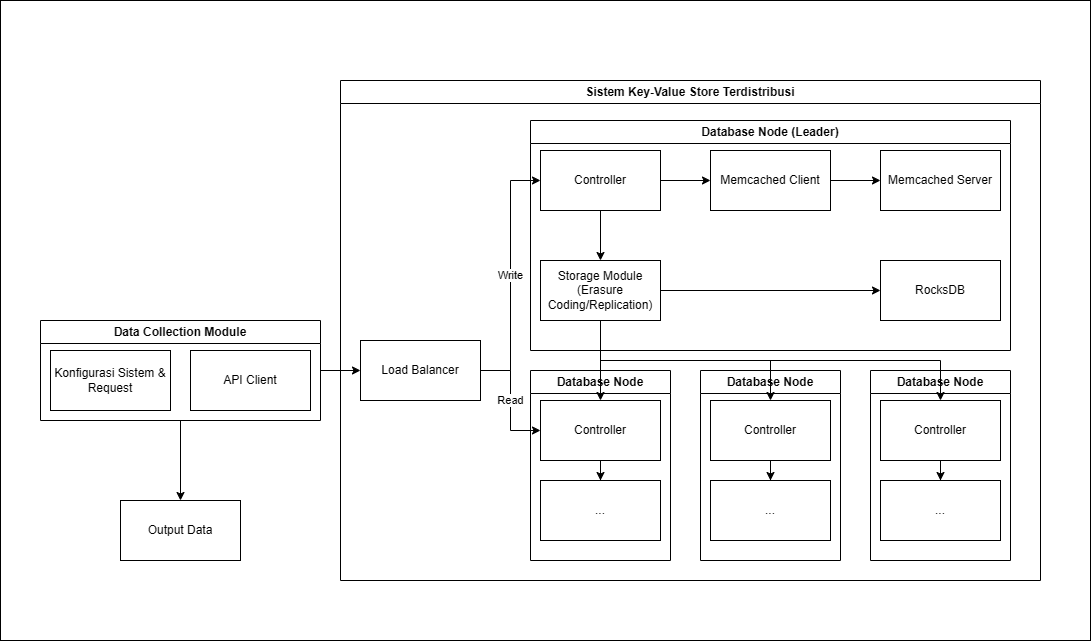
\includegraphics[width=0.95\textwidth]{resources/chapter-3/general-architecture.png}
    \caption{Struktur Subsistem Kontrol}
    \label{fig:control-subsystem-structure}
\end{figure}